\section{Kalibrierung des Torsions-Magnetometers}

Die Messwerte der Kalibrierungsmessung sind in Abbildung \ref{fig:MPKalibrierung} zu sehen. Zur Auswertung wird zunächst der durch die Spulen fließende Strom mit dem Spulenkennwert $s$ und der Formel
\begin{equation}
 B=s\cdot I=I\cdot \eb{26,5}{nT}{mA} 
\end{equation}
in das Magnetfeld umgerechnet. Der Plot der Messwerte und der linearen Regression ist in Abbildung \ref{fig:kalibrierung} zu sehen. Bei der Regression ergab sich eine Steigung von $\eb{-0.0039}{Skt}{nT}$. Der negative Kehrwert dieser Steigung liefert den Kalibrierungsfaktor
\begin{equation}
 \frac{\tau}{|\vec{m}|}=\eb{253}{nT}{Skt} \fullstop
\end{equation}

\begin{figure}
 \centering
 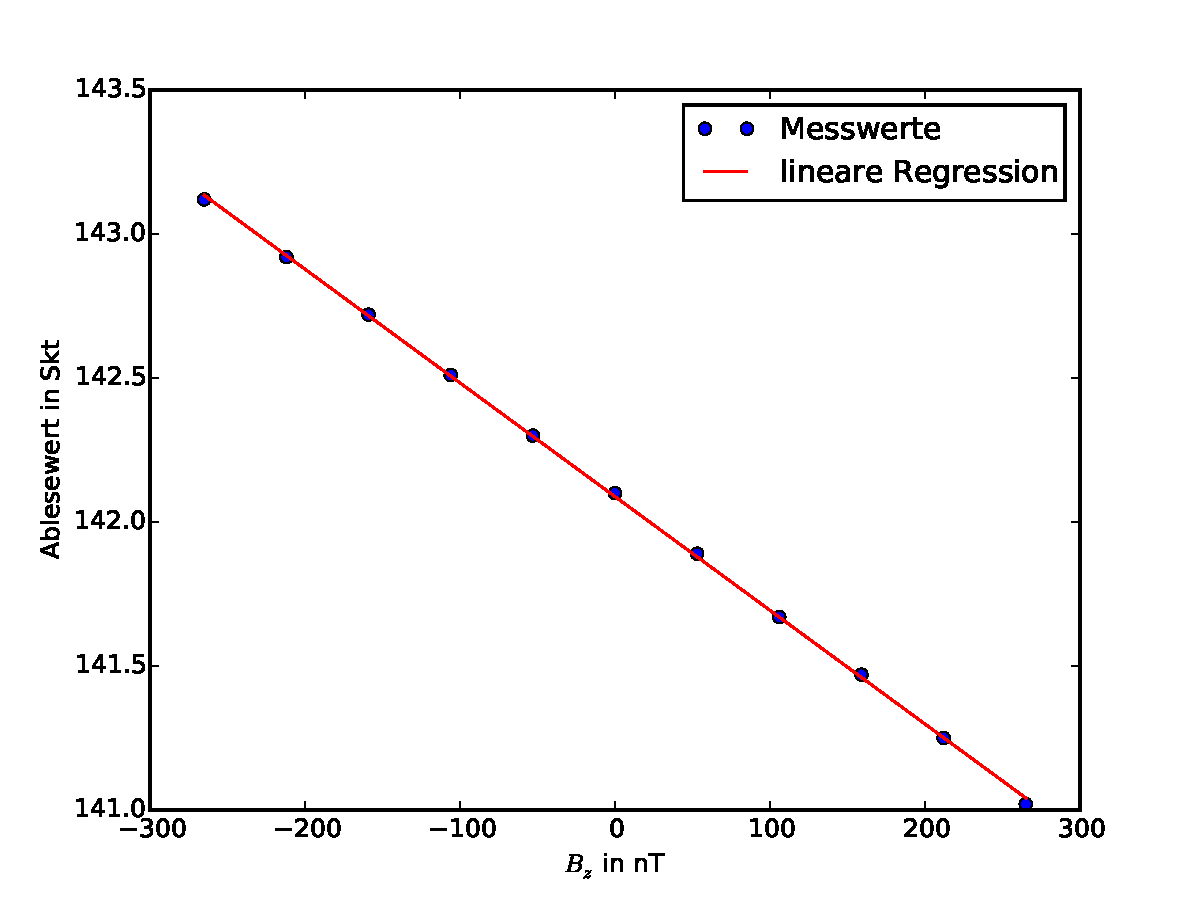
\includegraphics[width=\textwidth]{fig/kalibrierung.pdf}
 \caption[Bestimmung des Kalibrierungsfaktors des Torsions-Magnetometers]{Bestimmung des Kalibrierungsfaktors des Torsions-Magnetometers. Aufgetragen sind die Ablesewerte am Gfz in Skt über die angelegte magnetische Flussdichte in nT}
 \label{fig:kalibrierung}
\end{figure}


% \begin{figure}
%  \centering
%  \includegraphics[width=\textwidth]{fig/}
%  \caption{}
%  \label{fig:}
% \end{figure}